%!TEX root = ../report.tex
\chapter{Feature extraction} % (fold)
\label{chap:feature_extraction}
\section{Introduction}
This chapter explains how the target object is detected in both images as a previous step for the 3D reconstruction explained in chapter \ref{chap:stereopsis}. The algorithm detailed here computes the correspondent points to be tracked in the acquired images necessary input for the triangulation process.
The tracking of the object is a function implemented inside the node "balltracker" explained in chapter \ref{chap:ros_nodes_structure}.

\section{Algorithm}

\subsection{Target definition}
A key step in the process of tracking and triangulating problems is to provide a marker with robust enough features that avoid matching problems derived from occluding edges, homogeneous areas or repetitive structures.
In the case of occluding edges, the main issue is that a point on the border of the marker for one camera usually matches a different one from the other camera (specially for round or cylindrical objects) due to the change on the perspective.
Furthermore, the problem with homogeneous areas is that all the patches of a smooth surface with a constant illumination look exactly the same and can be mismatched.
Finally, the problem of repetitive surfaces affects mainly when it comes to matching images containing structures like fences or buildings which are usually very repetitive and can lead to mismatch features because they look too similar.

To avoid these problems, it was decided to use a sphere as a target object for detecting its center of mass.
The reason is that the surface of the ball, which is thus the feature used for detection, can be seen equally from both cameras disregarding their orientation.
Proceeding this way, the difficulties related to occluding edges and homogeneous surfaces can be avoided.
What is more, the ball itself is not a repetitive structure, so that it does not produce a problem either and can be easily extracted from the background.

\subsection{Image processing}
To achieve a reliable detection of the target in both images it was decided to use the contours finder provided by OpenCV.
The necessary binary images input to the finder, according to \cite{suzuki}, are obtained thresholding in HSV.
This is due to the fact that it turned out that the target color is easier to define in HSV than RGB, so that a robust, light invariant threshold can be computed and applied. The resulting image can be seen in figure \ref{fig:binary_image}.
However, this process yields some artifacts in the image which need to be removed for the contour finder not to detect too many unnecessary contours.

\begin{figure}[!ht]
    \centering
    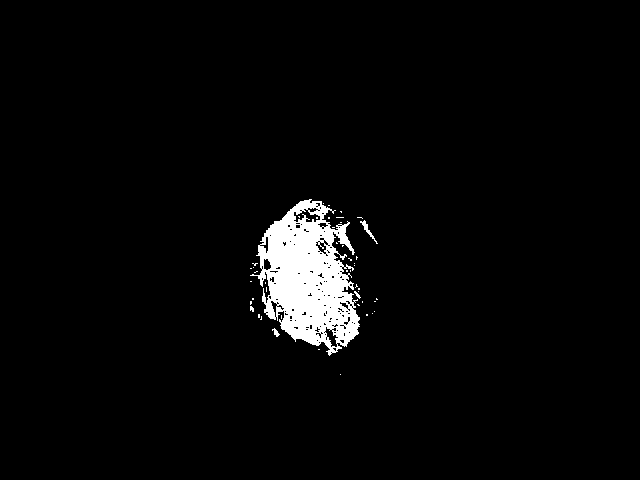
\includegraphics[width=0.8\textwidth]{images/binary.png}
    \caption{Binary image obtained after applying color threshold}
    \label{fig:binary_image}
\end{figure}

To filter out these artifacts two morphological operators are applied. First of all an opening operation with a square kernel of 9x9 pixels which removes the small blobs spread across the image and keeps the target intact. After, a closing operation is performed with the same kernel. The aim of this step is reducing the size of the gaps that appear inside the target after the thresholding in order to get a solid object. The result of the process can be seen in figure \ref{fig:filtered_image}.

\begin{figure}[h]
    \centering
    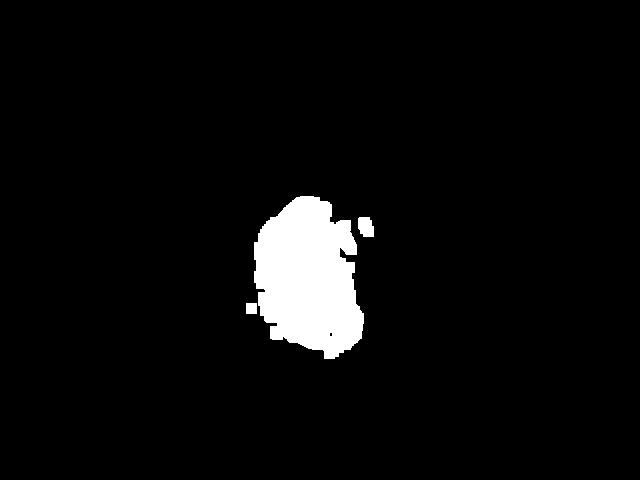
\includegraphics[width=0.8\textwidth]{images/filtered.png}
    \caption{Binary image obtained after applying the morphological operations}
    \label{fig:filtered_image}
\end{figure}

After removing the smallest objects from the binary image and closed the gaps in the remaining ones the finding contours function is applied, obtaining an array with the detected contours. Following, the area and the outer perimeter of all the contours are computed. With these values, a radius threshold, $r_\mathrm{threshold}$, is applied so that only the contours with enough radius are accepted. To do so, the equations for the perimeter and the area of a circumference are applied as it can be seen in equations \ref{eq:circ_perimeter} and \ref{eq:circ_area}.

\begin{equation}
\mathrm{perimeter}_\mathrm{contour} > 2 \pi r_\mathrm{threshold}
\label{eq:circ_perimeter}
\end{equation}

\begin{equation}
\mathrm{area}_\mathrm{contour} > 2 \pi r_\mathrm{threshold}^{2}
\label{eq:circ_area}
\end{equation}

Following, the circularity of the contours that have a radius bigger than the specified threshold is computed according to equation \ref{eq:circularity}, which gives a value between 1 and 0 (being 1 a perfect circle, and 0 a straight line). Having this value computed, a threshold for the circularity is set so that only the target passes it. Finally, the moments, $m$, of the remaining contour (the target) are calculated so that the centroids can be computed according to equation \ref{eq:centroids}. Then, these values are returned so that the stereopsis function can compute the 3D points of the target.

\begin{equation}
\mathrm{circularity} = \frac{4 \, \pi \, \mathrm{area}_\mathrm{contour}}{\mathrm{perimeter}_\mathrm{contour}^{2}}
\label{eq:circularity}
\end{equation}

\begin{equation}
\mathrm{centroid}_{X} = \frac{m_{10}}{m_{00}} \qquad \mathrm{centroid}_{Y}=\frac{m_{01}}{m_{00}}
\label{eq:centroids}
\end{equation}

\subsection{Dealing with illumination}
The main difficulty faced during the development of the target detection turned out to be the existing illumination in the workcell.
The position of the windows of the workspace and the changing intensity of the incoming natural light were the reasons to chose the final color of the marker and the approach taken for the algorithm.
The reflection of the light on the marker produced very bright spots on its top, preventing any other kind of target detection tried, for instance, based on shape extraction.
In addition, the walls surrounding the workcell are mainly white and, at certain moments of the day very bright.
To solve this issue, the ball was covered with a piece of green paper that made the color detection easier. Nevertheless, the high inclination of the sun still produced a spot of higher brightness in the top of the ball that wasn't detected by the algorithm. For fixing this, the closing morphology operation was performed as explained in the section above, which provided a much circular shape to the ball in the image than the one obtained by simply thresholding.

\section{Results}
Several variations of the algorithm stated above were tested before ending up with the presented one.
All in all, the final detection of the ball was stable enough to provide consistent data for the triangulation and the trajectory prediction.

% chapter feature_extraction (end)~\ref{sec:}